\documentclass[a4paper]{llncs}

\usepackage{xcolor}
\usepackage{amsmath} 
\usepackage{hyperref}
\usepackage{graphicx}
\usepackage{subcaption}

\hypersetup{
    colorlinks=true,
    linkcolor=magenta,
    urlcolor=blue,
    breaklinks,
    citecolor=blue
}


\newcommand{\bracketR}[1]{\left(#1\right)}
\newcommand{\bracketS}[1]{\left(#1\right)}
\newcommand{\bracketC}[1]{\left(#1\right)}
\newcommand{\innerproduct}[1]{\left<#1\right>}
\newcommand\norm[1]{\left\lVert#1\right\rVert}


\newcommand{\guy}[1]{\marginpar{\textcolor{orange}{Guy: #1}}}

\begin{document}


\title{Verifying the Resilience of Neural Network Watermarking}

\author{
  Ben Goldberger\inst{1} \and
  Yossi Adi\inst{2} \and
  Joseph Keshet\inst{2} \and
  Guy Katz\inst{1} 
}

\institute{
  The Hebrew University of Jerusalem, Israel \\
  \{jjgold, guykatz\}@cs.huji.ac.il
  \and
Bar Ilan University, Israel \\
\{a, b\}@biu.ac.il
}

\maketitle

\section{Introduction}

% Each of these should be extended into 1-2 paragraphs

Deep Neural Networks (DNN) are a nowadays phenomena in research and in Industry; They're used for large verity of applications, and achieving state of the art result in many fields (Computer vision, speech recognition, AI, and many more). DNNs flexibility and diversity are pushing the limits on what is possible for a computer to solve efficiently. As a result from their empiric success DNNs are now changing the way software is being designed, and broaden the role of Machine Learning trained functions in applications.

Because of the success of DNNs and because designing and training a DNN require certain expertise, time and processing power, the demand for a specifically designed DNN is growing, And Machine Learning as a Service (MLaaS) is now a thing. There are many machine learning services appearing in many forms, from data visualization and cloud computing to frameworks and semi-trained DNNs. This create some issues regarding the rights and ownership of some part of a trained network or design. Because of the relatively simple components of a DNN (Matrices, vectors and simple functions) it's quite easy to copy or use without permission.

In order to deal with such issues we need a way to authenticate a DNN. This may sound simple but the authentication needs to be robust, such that it's hard to remove. Here comes the concept of Digital Watermarking, a way of signing some Digital property such that it's hard to remove the signature, and said signature is unique. There are some proposed method of watermarking a DNN, but it's unclear how effective they are, meaning how difficult it is to remove the watermark from the DNN and what is the effect of removing the watermark.

DNN verification is a new and promising field. We propose a novel
methodology to use verification to measure and verify the robustness
of watermarking techniques.
Main uses of our approach: verify watermarked networks, assess
efficiency of watermarking schemes.

The rest of this paper is organized as follows. In
Section~\ref{sec:background} we provide the necessary background on
DNNs, watermarking, and DNN verification. Next, in
Section~\ref{sec:verifyWatermarks} we introduce our technique for
casting the watermark resilience problem into a verification
problem. Section~\ref{sec:evaluation} describes our implementation and evaluation of the approach on several watermarked DNNs for image
recognition. We discuss related work in Section~\ref{sec:relatedWork},
and conclude in Section~\ref{sec:conclusion}.

\section{Background}
\label{sec:background}

\cite{KaBaDiJuKo17Reluplex,KaHuIbJuLaLiShThWuZeDiKoBa19Marabou}

\section{Finding the minimal change that will get rid of the network's WaterMark}
\label{sec:verifyWatermarks}

Given a watermarked trained neural network as described
here \cite{AdBaPiKeWatermarking}.
\guy{make this a proper citation}
We
tested what is the minimal change to the network last layer in order
to "remove" some watermarks from the network.


\subsection{Defining the problem}
\label{sec:defineProblem}

Given a neural network $N$ with an output size $m$ the network
decision for an input $x$ is defined as the coordinate with the
maximal value, if the network output is the vector $y$ the decision is
$argmax_{i\in \bracketsS{m}} \bracketsC{y_i}$
\\\\
Given a watermarked network $N$ with a set of $K$ watermarks (A set of
inputs to the network) $\bracketsC{x_1,\cdots,x_K}$ we'll mark the
network last layer $L$ such that $L$ is a $m\times n$ matrix were $n$
is the layer's number of neurons and $m$ is the network output size.
The change to the last layer will be a matrix with the same dimension
as $L$ we'll mark as $\varepsilon$, such that $\varepsilon_{i,j}$ is
the change to the last layer matrix entry $L_{i,j}$. Well measure the
overall change to the layer as
$\norm{\varepsilon}_{\infty} =
max_{i,j}\bracketsC{\abs{\varepsilon_{i,j}}}$.
\\\\
For a certain input $x$ we're only interested in the input to the last
layer we'll mark the input to the last layer $v$. $v$ is a $n\times 1$
vector.  So the original network output $y = Lv$ and the changed
network output is $y' = (L+\varepsilon)v$. For a single input $x$ we
need to find the minimal $\varepsilon$ so that the
$argmax_{i\in\bracketsS{m}}\bracketsC{y_i}\neq
argmax_{i\in\bracketsS{m}}\bracketsC{y'_i}$
\\\\
Denote $d := argmax_{i\in \bracketsS{m}} \bracketsC{y_i}$ \\
For some $d'\in\bracketsS{m},d'\neq d$ finding $\varepsilon$ with
minimal $\norm{\varepsilon}_{\infty}$ such that
$y' = (L+\varepsilon)v\,$ and
$\,d' = argmax_{i\in\bracketsS{m}}\bracketsC{y'_i}$ can be described
in a Linear Programming form like so:

\begin{align*}
    Minimize:\quad & c \\
    Subject\ to:\quad & \forall i,j\quad -c \leq\varepsilon_{i,j}\leq c\\
    & y'=(L+\varepsilon)v \\
    & y'_d \leq y'_{d'}\\
\end{align*}
\hspace*{5cm} *The variables are the entries in $\varepsilon$ and $y'$
\\\\
Using the same method we can find how to change the network to more than one input.\\
Given inputs $x_1,\cdots,x_k$ and their respective inputs to the last layer $v_1,\cdots,v_k$ and their respected outputs and decisions $\bracketsC{y_1,\cdots,y_k}\ \bracketsC{d_1,\cdots,d_k}$ we want to find $\varepsilon$ such that\\
$\forall 1\leq j\leq k\quad d_j \neq argmax_{i\in\bracketsS{m}}\bracketsC{\bracketsR{\bracketsR{L+\varepsilon}v_j}_i}$\\
Assuming we choose our new desired output
$\bracketsC{d'_1,\cdots,d'_k}$
And now our LP looks like this:\\
\begin{align*}
    Minimize:\quad & c \\
    Subject\ to:\quad & \forall i,j\quad -c \leq\varepsilon_{i,j}\leq c\\
    & \forall j\quad y'_j=(L+\varepsilon)v_j \\
    & \forall j\quad \bracketsR{y'_j}_{d_j} \leq \bracketsR{y'_j}_{d'_j}\\
\end{align*}
\hspace*{5cm} *The variables are the entries in $\varepsilon$ and
$y'_j$
\\\\
Using
\href{http://aisafety.stanford.edu/marabou/MarabouCAV2019.pdf}{Marabou}
we can solve for the minimal $\varepsilon$ under different norm
$\norm{\varepsilon}_1=\sum_{i,j}\abs{\varepsilon_{i,j}}$ since using
this norm gives us a piece-wise linear problem.

\guy{Overall, this looks good. Some stuff will need to be moved to other
sections according to the paper layout.}

\section{Evaluation}
\label{sec:evaluation}
We tested this approach on a Neural network trained on the MNIST data set, the network was watermarked with $100$ images of Gaussian noise. The original network had $96.8\text{\%}$ accuracy on the MNIST test set and $100\text{\%}$ accuracy on the watermark images.

\begin{figure}[h!]
  \centering
  \begin{subfigure}{0.4\linewidth}
    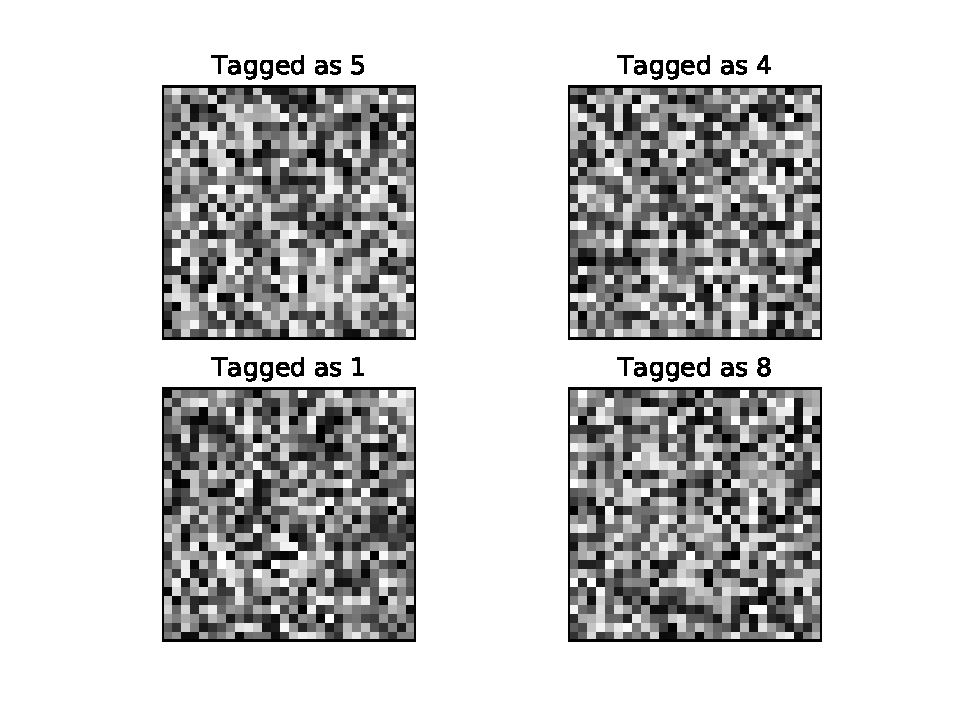
\includegraphics[width=\linewidth]{../data/wm.pdf}
     \caption{Water marks images.}
  \end{subfigure}
  \begin{subfigure}{0.4\linewidth}
    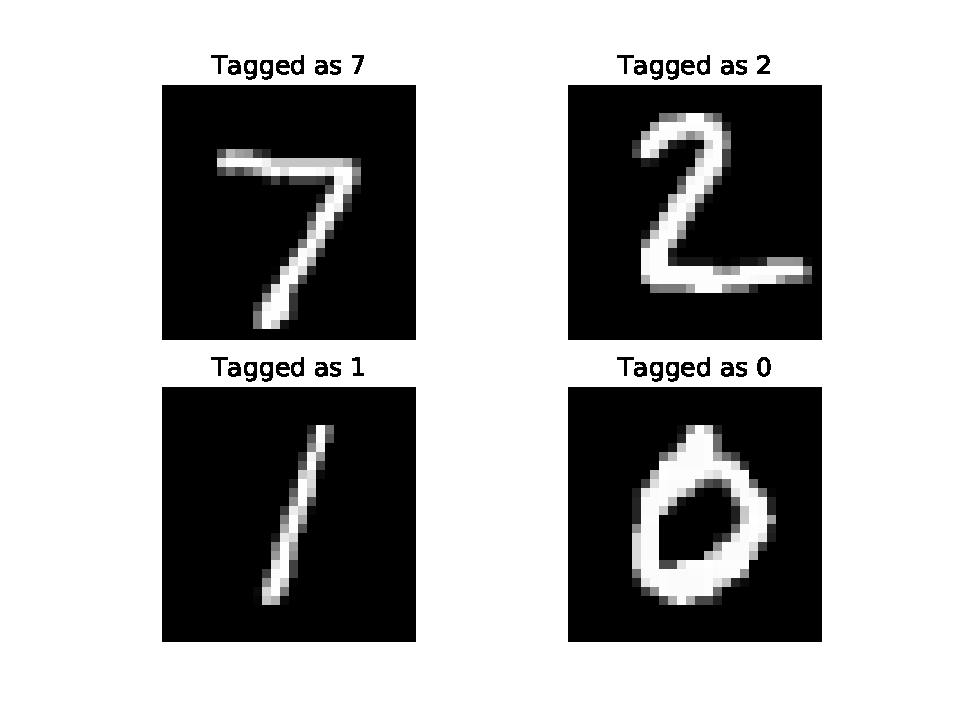
\includegraphics[width=\linewidth]{../data/mnist.pdf}
    \caption{MNIST images.}
  \end{subfigure}
  
  \label{fig:imageExamples}
\end{figure}

\subsection{Removing a single watermark}
The first test we did was to find the minimal change according to $\norm{\cdot}_{\infty}$ norm and $\norm{\cdot}_1$ norm for every water mark image as describe~\ref{sec:defineProblem}. We choose to change the original tagging of the image to the second highest score that image got. For example an image $w$ with an output $y$ 
$$j=\underset{i\in\bracketsC{0,\cdots,9}}{argmax}\bracketsC{y_i}$$ 
$j$ is the original tagging of $w$. 
$$j'=\underset{i\in\bracketsC{0,\cdots,9}\setminus \bracketsC{j}}{argmax}\bracketsC{y_i}$$ 
$j'$ is the new tagging of $w$. \\\\
meaning that after we change the last layer of the network the new output $y'$ largest coordinate is $j'$.   
Each watermark image have different minimal $\varepsilon$. This can give us some measure of how difficult it is to remove a single watermark image.

\begin{figure}[h!]
  \centering
  \begin{subfigure}{0.4\linewidth}
    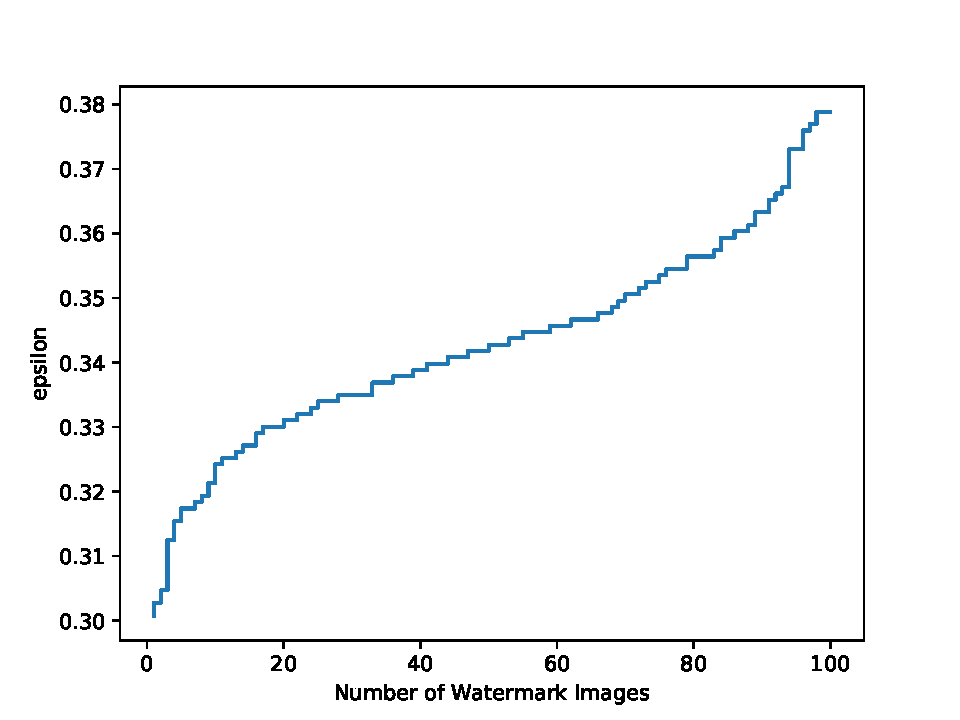
\includegraphics[width=\linewidth]{../data/results/problem1/mnist_w_wm.pdf}
     \caption{The Minimal $\norm{\cdot}_{\infty}$ for every watermark image}
  \end{subfigure}
  \begin{subfigure}{0.4\linewidth}
    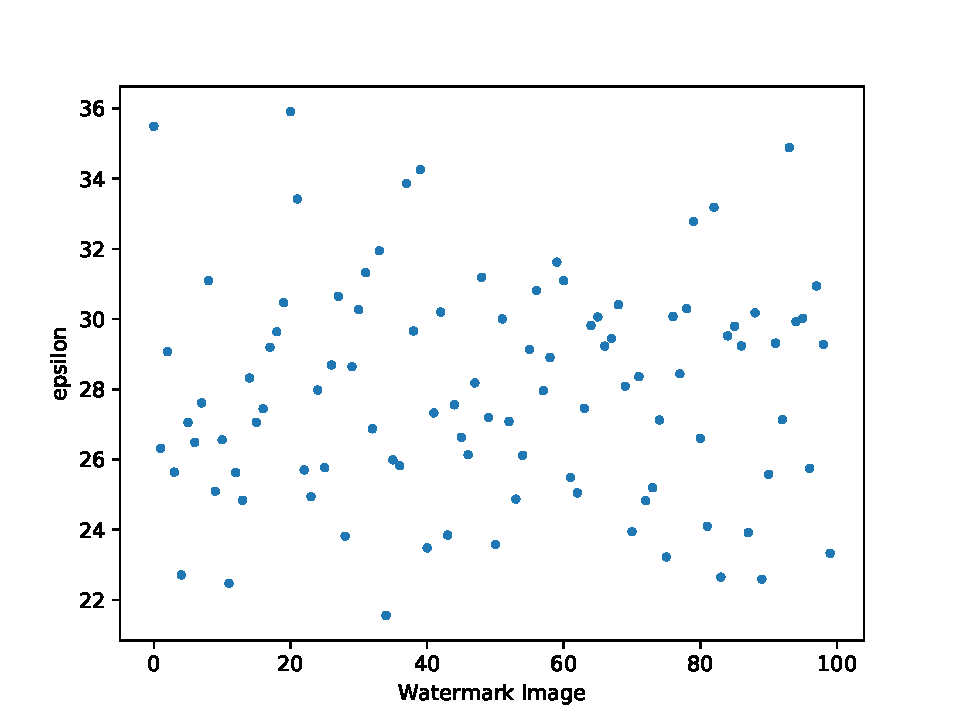
\includegraphics[width=\linewidth]{../data/results/problem2/mnist_w_wm.pdf}
    \caption{The Minimal $\norm{\cdot}_1$ for every watermark image}
  \end{subfigure}
  \label{fig:minimalEpsilonSingle}
\end{figure}

\subsection{Removing Multiple watermark}

Removing a single 


\section{Related Work}
\label{sec:relatedWork}

\section{Conclusion and Future Work}
\label{sec:conclusion}


\bibliographystyle{abbrv}
\bibliography{watermarks}

\end{document}

%%% Local Variables:
%%% mode: latex
%%% TeX-master: t
%%% End:
